\section{Introduction}

\begin{figure*}
	\centering
	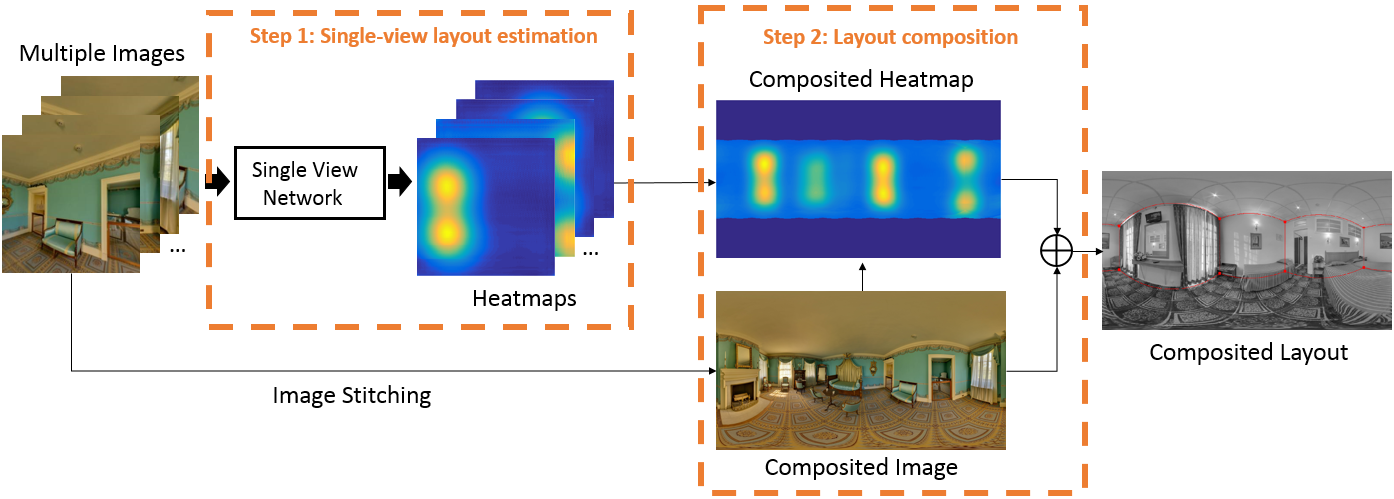
\includegraphics[width=\linewidth]{figs/ppline.png}
	\caption{Our pipeline consists of two main steps. First, a single-view network is employed to estimate the heatmap of room corners for each image separately. Secondly, the heatmaps of the input multi-view images are composed together to generate a combined heatmap of the room corners according to the image transformations. The final result is obtained by selecting the corners of local maximum.
		 }
	\label{fig:overview}
\end{figure*}

Indoor scene understanding has attracted wide attention due to its promising applications, including augmented/virtual reality and robotics. Massive researches have been carried out in related fields, such as semantic segmentation, room layout estimation and object detection. 
Room layout estimation is a fundamental task within scene understanding. It aims to predict the semantic boundaries between walls, the ceiling and the floor in a room. 
Since man-made indoor environments naturally follow some geometrical rules, for example objects always rest on the floor and many of them tend to be aligned with walls, the estimated room layout can provide valuable geometric priors, which can be applied in depth estimation, object detection~\cite{hedau2010thinking}, scene reconstruction \cite{lee2017joint} and so on.

%\xj{Traditional methods...}
Traditional approaches to this task usually follow a common proposing-ranking scheme \cite{hedau2009recovering,wang2013discriminative,gupta2010estimating,hedau2010thinking}. In the proposing stage, numerous layout hypotheses are obtained through vanishing point detection and ray sampling. Then, different hand-crafted features are used to find the best layout. 
\comments{
\xj{However, these techniques usually suffer from tedious and fragile post-processing tricks.}
\drf{It's the characteristic of DNN based method excluding \cite{zhao2017physics}}
}
With the rapid development of deep neural networks, recent methods built on fully convolutional network (FCN) have achieved remarkable performances in single-view images~\cite{mallya2015learning,dasgupta2016delay,ren2016coarse,zhao2017physics,LeeRoomNet17}. These networks efficiently learn object appearances and spatial distributions from a large database, and they implicitly encode these priors in the trained models to efficiently infer the layout of a new image. 
%\xj{limitations of single-view layout estimation techniques?}
%\xj{ambiguity of vertical walls, occluded corners.. multiple topology.}
%
However, these techniques usually suffer from tedious and fragile post-processing tricks. At the same time, single-view layout estimation has several inherent limitations, such as the ambiguity among walls claimed by \cite{dasgupta2016delay}, and the occlusion of critical semantic corners in a specific view. These limitations lead to non-perfect results that are still far from the requirements of practical applications.

%
While most of the previous work focused on estimating the room layout from one single-view image, we take more views into consideration. Unlike the single-view-based methods, the images taken from multi-views complement each other, which can ease the ambiguity caused by cluttered objects and occlusions of the room corners. At the same time, the combined room layout integrated from different views possess larger field of view (FOV) than that of the single-view layout. 
%
Few research has been carried out on multi-view-based layout estimation. \cite{bao2014understanding} follows the traditional proposing-ranking scheme in single-view layout estimation and merge the information from different views by integrating the structure from motion (SFM) into the framework. Their ranking part is implemented with complex hand-crafted features. 
%
In contrast, we propose a highly concise representation and an efficient algorithm to estimate the combined room layout from multi-view images.

%
Our work is similar in a sense to panorama-based room layout estimation \cite{zhang2014panocontext,zou2018layoutnet}. While we both explore a wider range of the room than a single shot, the panorama-based methods aim to recover the entire room structure in a \ang{360} panorama. 
%
\cite{zhang2014panocontext} presents a whole-room 3D context model which take a \ang{360} panorama as input and then outputs the detected objects and room layout. 
They extend the techniques used in single-view images by projecting the panorama into multiple perspective images first. 
In a subsequent technique \cite{zou2018layoutnet}, Zou et al. propose the LayoutNet network which are trained directly on panoramas to estimate the 3D room layout. They achieve better performance than \cite{zhang2014panocontext} in both accuracy and speed.
%
Inspired from these panorama-based methods, we design a new representation for room layout. Given multiple perspective images that are taken from different angles, we obtain a combined room layout at any FOV including the panoramic layout. Our approach also allows to revisit the same area several times because of the overlaps among multi-view images, which can enhance the prediction of interested space.

%
In order to reduce the ambiguities of different types of room layout, we propose a concise corner-based representation of room layouts in single-view image and design a single-view network to estimate these new corner-based layouts. 
The new representations of multiple views are easy to integrate.
We combine the estimated room layouts from different perspectives and generate a combined room layout using weighted average in the overlapping area. 
The final results look reasonable and impressive. 
We also evaluate our approach quantitatively on a panorama dataset and achieve comparable performance on whole-room layout with full \ang{360}-panorama-based methods without losing the flexibility.   

\comments{
To make full use of the contextual information for better understanding of an indoor scene, \cite{panocontext} present a whole-room 3D context model which take a \ang{360} panorama as input and then output the detected objects and room layout in 3D. They extends the techniques used in single-view images by projecting the panorama into multiple overlapping perspective images first. In a subsequent technique \cite{LayoutNet}, Zou et al. propose the LayoutNet network which trained directly on the panoramic images to estimate the 3D room layout. They achieve better performance in both accuracy and speed. However, it is not always convenient to obtain high-quality \ang{360} panoramic images that requires no position change between cameras in many applications. 
For this reason, we propose to explore the whole room structure using multi-view images \xj{that can be taken under different angles and locations} (if we know the camera position, yes) as an alternative scheme.

(add intro for multi-view layout estimation, there are two related papers using SFM) \xj{And compare our method with them.}
\xj{Emphasize our contribution and novelty here. }

By representing the entire room with multi-view images, we can naturally benefit from the mature techniques on perspective images. The estimated room layouts from different views can supplement each other and further improve the prediction accuracy of each perspective. Then we merge the prediction from multiple overlapping images and produce the holistic estimation of layout. The 3D structure of the entire room can be reconstructed from our holistic prediction, as depicted in Fig. \ref{fig:renderingResults}.
}


